

\documentclass{resume} % Use the custom resume.cls style

\usepackage[left=0.75in,top=0.6in,right=0.75in,bottom=0.6in]{geometry} % Document margins
\usepackage{hyperref}
\usepackage{graphicx}
\usepackage{wrapfig}
\name{Y Narasimhulu} % Your name
\address{Research Scholar \\ University of Hyderabad} % Your address
\address{(+91)~$\cdot$~970~$\cdot$~363~$\cdot$~1188 \\ narasimedu@gmail.com \\ 18mcpc17@uohyd.ac.in} 
% Your phone number and email

\begin{document}

\makebox[\textwidth]{ GitHub: \href{https://github.com/Narasim}{https://github.com/Narasim}} 
%----------------------------------------------------------------------------------------
%	EDUCATION SECTION
%----------------------------------------------------------------------------------------

\begin{rSection}{Education}
	
\begin{rSubsection}{Ph.D.}{Pursuing}{}{}	
	\item Pursuing Ph.D. at \textbf{School of Computer and Information Sciences(SCIS), University of \\ Hyderabad}, Hyderabad.(Almost at the ending stage) \\
	\textbf{Thesis Title}: Design, Study, and Analysis of Classification Algorithms.
\end{rSubsection}

\begin{rSubsection}{M.Tech}{}{}{}%{2009 - 2011}{}{}	
	\item Post Graduation (Computer Science), from \textbf{St.John's College of Engineering and Technology}, Yemmiganur.
\end{rSubsection}

\end{rSection}


%----------------------------------------------------------------------------------------
%	ACHIEVEMENTS SECTION
%----------------------------------------------------------------------------------------

\begin{rSection}{ACHIEVEMENTS}
	\begin{rSubsection}{}{}{}{}	
		\item[.] Member of a winning team from the University of Hyderabad: Cardiff University's CyberAI Research Challenge in collaboration with the University of Hyderabad and Osmania University. \\\textbf{Title}: Privacy Preserving Federated Learning on Healthcare Data \\Further extending this work into a Journal Publication.
	\end{rSubsection}
	\begin{center}
		\begin{tabular}{||>{\rule[-1.3ex]{0pt}{4ex}}c c c c||}
			\hline
			\textbf{S.No.} & \textbf{Board and Exam} & \textbf{Award} & \textbf{Qualifying Year} \\ [0.5ex] 
			\hline\hline
			1 & UGC - NET & Junior Research Fellow(JRF) & July - 2018 \\ 
			\hline
			2 & UGC - NET & Assistant Professor & July - 2018 \\
			\hline
			3 & UGC - NET & Assistant Professor & December - 2017 \\
			\hline
			4 & UGC - NET & Assistant Professor & June - 2014 \\
			\hline
			5 & GATE & Computer Science & 2019 \\ [1ex] 
			\hline
		\end{tabular}

	\end{center}
	
	
\end{rSection}



%----------------------------------------------------------------------------------------
%	TECHNICAL STRENGTHS SECTION
%----------------------------------------------------------------------------------------
\begin{rSection}{Research Experience}
	
	\begin{rSubsection}{}{}{}{}	
		\item[.] A \textbf{Senior Research Fellow} from January 2021 to Present at University of Hyderabad.
		\item[.] A \textbf{Junior Research Fellow} from January 2019 to December 2020 at University of Hyderabad.
		
	\end{rSubsection}	
	
\end{rSection}
\begin{rSection}{Research Interests}
	
	\begin{tabular}{ @{} >{}l @{\hspace{6ex}} l }
		 $\cdot$ Clustering & $\cdot$ Classification \\
		 $\cdot$ Nearest Neighbors & $\cdot$ Deep Learning\\
		 $\cdot$ Matrix Approximations & $\cdot$ Optimization Algorithms
		
	\end{tabular}
	
\end{rSection}




%----------------------------------------------------------------------------------------
%	WORK EXPERIENCE SECTION
%----------------------------------------------------------------------------------------


%\begin{rSection}{Professional Affiliations}
%	
%	\begin{rSubsection}{}{}{}{}	
%		\item Life Long Member of Indian Society for Technical Education(ISTE).
%	\end{rSubsection}
%	
%	
%\end{rSection}
\begin{rSection}{Certifications}
	
	\begin{rSubsection}{}{}{}{}
		\item \textbf{``Foundations of Data Science"},  by One Fourth Labs - Mitesh M Khapra, and Pratyush Kumar, IIT Madras Research Park.
		\item \textbf{``Deep Learning"}, by One Fourth Labs - Mitesh M Khapra, and Pratyush Kumar, IIT Madras Research Park.
		
	\end{rSubsection}
	
\end{rSection}


\pagebreak

\begin{rSection}{Papers Published/Under Review}
	
	\begin{rSubsection}{}{}{}{}
		
		\item[1] \textbf{Y Narasimhulu, V China Venkaiah, ``ActiveSVM: An Active Learning Algorithm With Novel Initialization, and SVM Model Update Techniques"}, Manuscript communicated to the Journal, Advances in Data Science and Adaptive Analysis, World Scientific. 
		
		\item[2] \textbf{Y Narasimhulu, Pralhad K, V China Venkaiah, ``Revisiting Winnow: A Modified Online Learning Algorithm for Efficient Binary Classification"}, Manuscript communicated to the Journal, Statistical Analysis and Data Mining, Wiley.
		
		\item[3] \textbf{Y Narasimhulu, V China Venkaiah, ``Low-rank Binary Matrix Approximation using SVD Based Clustering Technique: Detecting Autism Spectrum Disorder (ASD)"}, accepted by SN Computer Science Journal, Springer Nature(Impact Factor: 3.78).
		
		\item[4] \textbf{Umesh Kumar, Y. Narasimhulu, V. Ch. Venkaiah, ``MQG-PRNG and Non-Associative Quasigroup based Stream Cipher"}, Communicated to a Journal.
		
		\item[5] \textbf{M. S. Raghavendra, P. Chawla and Y. Narasimhulu, ``A Probability Based Joint-Clustering Algorithm for Application Placement in Fog-to-Cloud Computing,"}, 2021 9th International Conference on Reliability, Infocom Technologies and Optimization (Trends and Future Directions) (ICRITO), Noida, India, 2021, pp. 1-5, doi: 10.1109/ICRITO51393.2021.9596534(SCOPUS Indexed).
		
		\item[6] \textbf{Y Narasimhulu, Ashok Suthar, Raghunadh Pasunuri, V China Venkaiah (2021), ``CKD-Tree: An Improved KD-Tree Construction Algorithm"}, Published in Proceedings of the \\ International Semantic Intelligence Conference 2021(ISIC 2021), CEUR Conference Proceedings(CEUR-WS.org)(SCOPUS Indexed: https://www.scopus.com/sourceid/21100218356).
		
		\item[7] \textbf{Narasimhulu Y, Pasunuri R., Venkaiah V.C. (2021), ``Nearest Neighbors via a Hybrid Approach in Large Datasets: A Speed up."}, In: Chaki N., Pejas J., Devarakonda N., Rao Kovvur R.M. (eds) Proceedings of International Conference on Computational Intelligence and Data Engineering. Lecture Notes on Data Engineering and Communications Technologies, vol 56. Springer, Singapore(SCOPUS Indexed: https://www.scopus.com/sourceid/21100975545).
		
		\item[8] \textbf{Vardhani P.R, Priyadarshini Y.I., Narasimhulu Y. (2019), ``CNN Data Mining Algorithm for Detecting Credit Card Fraud."}, Published in Soft Computing and Medical Bioinformatics. SpringerBriefs in Applied Sciences and Technology. Springer, Singapore(Web of Science Indexed: https://www.webofscience.com/wos/woscc/full-record/WOS:000445142100010).
		
		\item[9] \textbf{K.Vinod Kumar Reddy, Y. Narasimhulu, ``Proficiently Sharing Data Using Name Based Routing Algorithm in Big Data."}, Published in International Journal of Trend in Research and Development (IJTRD), ISSN:2394-9333, Special Issue - RIET-17 , December 2017(UGC-Care List).
	\end{rSubsection}
	
	
\end{rSection}

\begin{rSection}{Current Works}
	
	\begin{rSubsection}{}{}{}{}	
		\item[.] A survey on various Online learning algorithms
		\item[.] Privacy Preserving Federated Learning
	\end{rSubsection}
\end{rSection}



\begin{rSection}{My Peer Reviews}
	
	\begin{rSubsection}{IEEE Access:}{}{}{}	
		\item[1] A K-Means-Based Interpolation Algorithm with Lp-Norm and Feature Weighting
		\item[2] Assessing Decision Tree Stability: A Com-prehensive Method for Generating a Stable Decision Tree
		\item[3] Credit card fraud detection based on improved Variational Autoencoder Generative Adversarial Network.
		\item[4] Revolutionizing Perimeter Intrusion Detection: A Machine Learning-Driven Approach with Curated Dataset Generation for Enhanced Security.
		\item[5] Integrating Unsupervised Clustering and Semi-Supervised
		Learning for Faulty Insulator Classification.
		\item[6] Hyper Robust H-infinity Filter and PSO-SVM Based Monitoring of Power Quality Disturbances system.
		\item[7] Anchor Pseudo-supervise Large-scale Incomplete Multi-view Clustering.
		\item[8] Mobility Data Science
		\item[9] High-Accuracy Feature-Centric COVID-19 Prediction Using Optimized Union Ensemble Approach
		\item[10] Distributed Feature matching for Robust Object Localization in Robotic Manipulation
	\end{rSubsection}
	\begin{rSubsection}{Neural Computing and Applications:}{}{}{}		
		\item[1] Streamlining Plant Disease Diagnosis with Convolutional Neural Networks and Edge	Devices.
	\end{rSubsection}
	\begin{rSubsection}{Soft Computing:}{}{}{}		
		\item[1] Multimedia Protection and Abnormal Behaviour Identification in SDN Using Cuckoo Search Based One Class Support Vector Machine.
	\end{rSubsection}
	 \href{https://www.webofscience.com/wos/author/record/IUN-0908-2023}{Reviews details can be found at: Web of Science} or \href{https://orcid.org/0000-0001-8482-7678}{ ORCID}
\end{rSection}




\begin{rSection}{Conferences Attended}
	
	\begin{rSubsection}{}{}{}{}
		\item \textbf{``ACM COMPUTE, Sixth Annual Conference"}, at University of Hyderabad, Hyderabad, India 2023. Also a volunteer in the organising committee.
		\item \textbf{``International Semantic Intelligence Conference(ISIC - 2021)"}, at MERI College of Engineering \& Technology, New Delhi, India 2021.
		\item \textbf{``Third International Conference on Computational Intelligence \& Data Engineering\\(ICCIDE - 2020)"}, at Vasavi College of Engineering(Autonomous), Hyderabad, Telangana, India 2020.
		\item \textbf{``Second International Conference on Cognitive Science and Articial Intelligance(ICCSAI - 2018)"}, at Sree Vidhyanikethan Engineering College(Autonomous), Tirupati, Andhra Pradesh India 2018.

	\end{rSubsection}

\end{rSection}


\begin{rSection}{Technical Strengths}
	
	\begin{tabular}{ @{} >{\bfseries}l @{\hspace{6ex}} l }
		$\cdot$ Computer Languages: & C, and Python \\
		$\cdot$ Programming & Numpy, Pandas, Keras \& sklearn
	\end{tabular}
	
\end{rSection}

\begin{rSection}{External Links}
	
	\begin{rSubsection}{}{}{}{}	
		\item[.] LinkedIn: \hspace{1.5cm} \href{https://www.linkedin.com/in/narasimhulu-yeggoli/}{https://www.linkedin.com/in/narasimhulu-yeggoli/}
		\item[.] GitHub: \hspace{1.8cm} \href{https://github.com/Narasim}{https://github.com/Narasim}
		\item[.] ORCID: \hspace{1.8cm} \href{https://orcid.org/0000-0001-8482-7678}{https://orcid.org/0000-0001-8482-7678}
		\item[.] Google Scholar:  \hspace{0.5cm}
		\href{https://scholar.google.com/citations?user=agFT18IAAAAJ\&hl=en}{https://scholar.google.com/citations?user=agFT18IAAAAJ\&hl=en}
		\item[.] LeetCode: \hspace{1.4cm} \href{https://leetcode.com/narasimhuluy/}{https://leetcode.com/narasimhuluy/}
		
		
	\end{rSubsection}	
	
\end{rSection}


%\begin{rSection}{Work Experience}
%	
%	\begin{rSubsection}{Assistant Professor}{June 2011 - October 2012}{1.4 Years}{}
%		\item Worked as ``ASSISTANT PROFESSOR" at St. JOHNS' COLLEGE OF ENGG. AND TECHNOLOGY
%	\end{rSubsection}
%	
%	%------------------------------------------------
%	
%	\begin{rSubsection}{Assistant Professor}{October 2012 - December 2018.}{6.2 Years}{}
%		\item Worked as ``ASSISTANT PROFESSOR" at RAVINDRA COLLEGE OF ENGINEERING FOR WOMEN
%	\end{rSubsection}
%	
%	
%	\begin{rSubsection}{Tutor}{December 2023 - Present}{}{}
%		\item Working as ``Tutor" at WIINGY an Online Tutoring Service.
%	\end{rSubsection}
%	%------------------------------------------------
%	
%\end{rSection}
%
%\begin{rSection}{Subjects Taught}
%	
%	\begin{tabular}{ @{} >{}l @{\hspace{6ex}} l }
%		$\cdot$ Design and Analysis of Algorithms & $\cdot$ Operating Systems\\
%		$\cdot$ Data Structures & $\cdot$ Database Management Systems\\
%		$\cdot$ Advanced Data Structures and Algorithms & $\cdot$ Java and Web Technologies\\
%		
%		$\cdot$ Web Programming
%		
%	\end{tabular}
%	
%\end{rSection}




\begin{rSection}{Campus Trainings Conducted}
	
	\begin{rSubsection}{}{}{}{}	
		\item 22 Days training on \textbf{`Data Structures and Algorithms'} at `Shri Ramdeobaba College of Engineering and Management', Nagpur, Maharastra.
		\item 15 Days training on \textbf{`Problem Solving Skills'} at Mohan Babu University(MBU), Tirupati.
%		\item An Andhra Pradesh State Skill Development Corporation 10 day training programme on \\ \textbf{`C-Programming and Computer Fundamentals'} at `Govt. Silver Jubilee College', Kurnool.
%		\item An Andhra Pradesh State Skill Development Corporation 10 day training programme on \\ \textbf{`C-Programming and Computer Fundamentals'} at `Sri Ramakrishna Degree College and National Degree College', Nandyal.
%		\item An Andhra Pradesh State Skill Development Corporation 1 day training programme on \\ \textbf{`C-Programming and Data Structures'} at `Chalapathi Institute of Engineering and Technology', Guntur.
		\item An Andhra Pradesh State Skill Development Corporation 2 day training programme on \\ \textbf{`C-Programming and Data Structures'} at `QIS College of Engineering \& Technology', Ongole.
		\item An Andhra Pradesh State Skill Development Corporation 1 day campus training programme on \textbf{`C-Programming and
		Data Structures'} at `QIS College of Engineering \& Technology', Ongole.
	\end{rSubsection}
	
	
\end{rSection}



%\begin{rSection}{Projects Worked - Excluding the works presented in the section `Papers Published'}
%	
%	
%	\begin{rSubsection}{DEEDSP: Deadline-aware and Energy-efficient Dynamic Service Placement in Integrated IoT and Fog Computing Environment}{}{}{}	
%		\item[] Fog computing has become adaptable and also as a promising infrastructure for providing elastic resources at the edge of the network. Fog computing reduces the transmission latency and consumption of bandwidth while processing the incoming requests from various Internet of Things (IoT) devices. Moreover, fog computing can support and facilitate geographically distributed applications with low and predictable latency. However, this technology also has significant research issues in its current stage. For example, whether a fog computing framework is suitable for implementing successful service location models could be an unresolved issue. We proposed a Deadline and Energy Efficient Dynamic Service Placement (DEEDSP) technique for fog computing that supports the placement of IoT based services. Further, hyper-heuristic algorithm based energy-efficient service placement technique is proposed to balance the energy-delay trade-off based on different service placement decision criteria (e.g., minimum response time or energy consumption). The proposed algorithm is able to minimize the energy consumption of the system dynamically while ensuring that the response time satisfies a given time constraint. Finally, proposed technique is evaluated in simulated fog computing environment and experimental results show that this technique performs better than state-of-the-art placement techniques in terms of energy and latency.
%		\\Meeniga Sri Raghavendra, Priyanka Chawla, and Sukhpal Singh Gill. 2021. DEEDSP: Deadline‐aware and energy‐efficient dynamic service placement in integrated Internet of Things and fog computing environments. Trans. Emerg. Telecommun. Technol. 32, 12 (December 2021). https://doi.org/10.1002/ett.4368 (Worked unofficially).
%	\end{rSubsection}
	
	
	
%\end{rSection}



\begin{rSection}{Declaration}
	
	\begin{rSubsection}{}{}{}{}	
		\item[] Hereby declare that the information furnished above is true.
	\end{rSubsection}

	\vspace{1cm}

	\begin{flushright}
		Y NARASIMHULU \\
		
\includegraphics[scale=0.75]{signature.jpg}
	\end{flushright}


\begin{figure}[!hbt]
		\begin{flushright}
			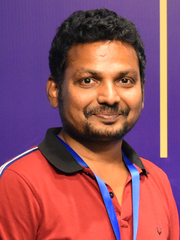
\includegraphics[width=0.2\textwidth]{Narasimpassport.png}
		\end{flushright}
\end{figure}

	
\end{rSection}
%----------------------------------------------------------------------------------------
%	EXAMPLE SECTION
%----------------------------------------------------------------------------------------

%\begin{rSection}{Section Name}

%Section content\ldots

%\end{rSection}

%----------------------------------------------------------------------------------------

\end{document}
